%!TEX root = cscw2018-comic.tex
\section{Study on Persiasion: Results}
\label{sec:Study on Behavior Results}

\subsection{Raw Data}
\label{sub:Study on Behavior Raw Data}
In total we have 307 participants joined our study, 101 participants received the message in the text form, 102 participants received the same message in the comic form, and 104 participants received the comic message with social-proof. We ran an outlier analysis on participants' completion time and removed 30 participants from our dataset. The following analysis is based on a dataset with 277 participants, 91 of them is in pure-text condition, 97 of them is in comic condition, and 92 of them is in comic-social-proof condition.

\subsection{Analysis}
\label{sub:Study on Behavior Analysis}

Similar as the first study on perference, we analyzed the data with Bayesian inference. The result ~\ref{fig:main-experiment2-effect} shows the effect size between abstract-comic v. pure-text = 0.47; There is no overlap of the 95 \% high probability density (HPD) interval with the ROPE of [-0.1, 0.1]). Thus the effect is significant; the effect size between abstract-comic and social-proof-comic is 0.13; but since the distribution includes a ROPE of $-0.1 \pm 0.1$, the effect is not significant.

\begin{figure*}
 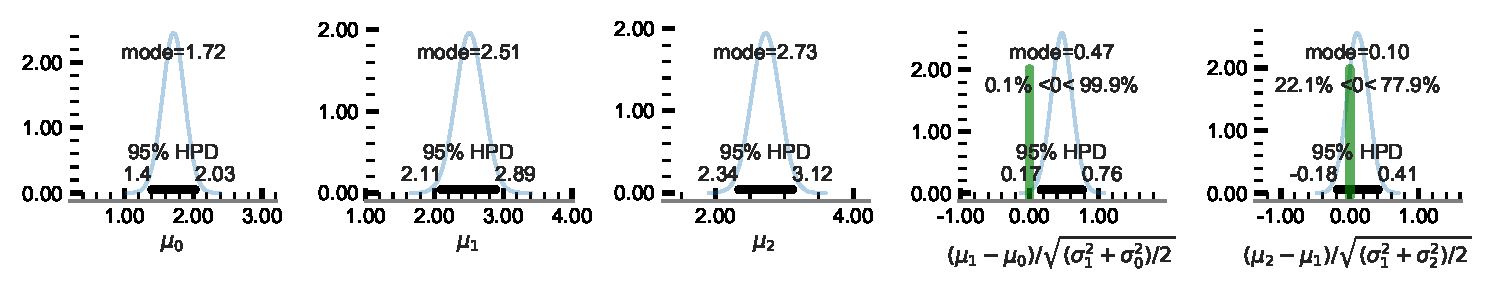
\includegraphics[width=1\textwidth]{./hari-code/new_exp_text_v_comic_v_social.pdf}
 \caption{The figure show the posterior distribution of the amount of money participants decide to donate $\mu_i$. and the contrast among conditions.}
 \label{fig:main-experiment2-effect}
\end{figure*}

In this section, we presented a Bayesian model to analyze the overall effect of using a abstract-comic to persuade people making charitable donation decisions, and understand the effect of adapting persuasive techniques in the abstract comic form. The results show that the use of abstract-comic produces a significant effect in persuading participants to donate. Although abstract-comic with social proof can produce larger effect, the contrast between abstract-comic and abstract-comic with social proof is not significant. Next we discuss the findings, including qualitative feedback from the participants.
